\documentclass[10pt,conference,compsocconf]{IEEEtran}
\usepackage{multirow}

\usepackage{amsmath}    % math
\usepackage{graphicx}   % For figure environment
\usepackage{todonotes}
\usepackage{subcaption}

\usepackage{hyperref}
\begin{document}
\title{Mini-project I}

\author{
  Luc\'{i}a Montero Sanchis, Milica Novakovi\'{c}, Ada Pozo P\'{e}rez,\\
  \textit{Deep Learning 2018, EPFL Lausanne, Switzerland}
}

\maketitle

\begin{abstract}
In this report we train a model based on LSTM and CNN for predicting the laterality of finger movements based on Electroencephalography (EEG) recordings. We evaluate the effect of preprocessing or not the data and compare the results obtained using a baseline model based on SVM, with accuracies up to 74\%, to the ones obtained using LSTM, CNN and our final model that combines LSTM and CNN architectures. These last two models are capable of outperforming the baseline, reaching 80\% accuracy, whereas the LSTM is not capable of modelling the data and obtains worse results. It is found that despite the noisy data found in EEG recordings, preprocessing is in general detrimental for models' performance and using raw input data should be preferred.

\end{abstract}

\section{Introduction}
In this project we train a predictor of finger movements from Electroencephalography (EEG) recordings using the PyTorch framework. The objective is to implement a neural network that predicts the laterality of the finger movement, i.e. if it corresponds to a right or left movement, from the EEG recording.

The difficulty to solve this kind of problems based on neuroimaging comes in general from the lack of large scale datasets \cite{BashivanRYC15}. This limited number of samples difficults training deep models with millions of parameters.


We attempt to tackle this problem using different models. First, we use Support Vector Machines (SVM) \cite{BashivanRYC15} as a baseline, which helps us assess the accuracy of models based on Long Short-Term Memory Unit (LSTM) \cite{BashivanRYC15, LSTM} and Convolutional Neural Network (CNN) \cite{BashivanRYC15, SchirrmeisterSF17}. Several experiments are conducted with these models, evaluating the results obtained under different conditions such as using the raw data or preprocessing it.


The rest of this paper is organized as follows: Section \ref{sec:database} describes the database and the preprocessing steps considered. The methods and architectures used are introduced in Section \ref{sec:methods}, while the results are presented and discussed in Section \ref{sec:results}. Lastly, conclusions are drawn in Section \ref{sec:conclusions}.

\section{Database}
\label{sec:database}
The database used is the dataset IV of the "BCI Competition II" \cite{data}. The training set is composed from 316 samples, whereas the test set has 100 test samples. The signals were recorded at 1 kHz during 0.5 seconds with a band-pass filter between 0.05 and 200 Hz. Each of them is composed of 28 EEG channels. 

In addition to the signals captured with 1 kHz sampling rate, this work also uses a version downsampled to 100 Hz.


\subsection{Preprocessing}
\label{ssec:preprocessing}

In general, EEG signals typically have low signal-to-noise ratio and suffer other interferences such as power line noise and artifacts from other muscles and eye movements \cite{SchirrmeisterSF17, LSTM, BashivanRYC15}. To overcome these problems we have investigated both filtering the signal and reducing the number of electrodes before using it as input to the network.

    \subsubsection{Filtering and normalization}
        \begin{itemize}
        
            \item Notch filter: A notch filter was applied to the frequency range of 50 Hz with a quality factor of $Q=30$  \cite{LSTM}. The  motivation was to reduce the power line noise  \cite{LSTM}. 
            \item High pass filter: The objective of this filter is to reduce artifacts that may have been produced by movements of the electrodes against the skin  \cite{LSTM}. This is implemented using a IIR Butterworth filter of order five with cutoff frequency of 0.5 Hz \cite{LSTM}.
            \item Standardization: After filtering, the EEG signals are normalized using standardization, that is, removing the mean and dividing by the standard deviation of each channel. 
        \end{itemize}
        Since in general the tendency with deep learning is to implement as little preprocessing as possible \cite{SchirrmeisterSF17}, the models will be evaluated with and without this filtering and  the resulting performances will be compared.
    \subsubsection{Reducing the number of electrodes}
    Having in mind that few brain areas are in charge of finger movements \cite{electrode}, we study whether the information from a couple of electrodes is enough to decode the finger movements. The motivation for this is that using only the electrodes that contain the most discriminant information about the movements could help reduce  the complexity of the models.
    
    We use Fisher distance to determine which electrodes are the most discriminant, keeping only the ones with values higher than a certain threshold. However, this simplification seems to be detrimental and reduces the performance in simple experiments. Hence, we consider all  electrodes in all the experiments explained in Section \ref{sec:results}.

\section{Methods} % (fold)
\label{sec:methods}
We attempt to solve the task presented using Support Vector Machines (SVMs) and deep neural networks with models based on Long Short-Term Memory Units (LSTMs) and Convolutional Neural Networks (CNNs).


\subsection{Support Vector Machines (SVM)}
\label{ssec:methods_SVMs}
SVMs try to find the hyperplane that best separates two classes by leaving the maximum margin from both of them. The margin is defined as the distance from the nearest point of each class to the hyperplane. In other words, the margin is the minimum distance between the hyperplane and each of the classes. 
 
% To develop complex non-linear classifiers SVM can be adapted using kernels. Kernels map the input $l$-dimensional feature space into a $k$-dimensional space where the input is linearly separable. 
 
 In this work we will use a linear kernel and a non-linear Radial Basis Function (RBF). The first one only has a regularization parameter $C$, which tends to reduce overfitting the smaller it is, whereas RBF also has the width of the Gaussian kernel $\gamma$ as parameter. A smaller $\gamma$ implies that the kernel varies more abruptly the kernel and thus the SVM will be more prone to overfit.
 
\subsection{Long Short-Term Memory Units (LSTM)}
\label{ssec:methods_LSTM}

\begin{figure}[t]
    \centering
    \includegraphics[width=\linewidth]{figures/LSTM_archi.pdf}
    \caption{Our architecture for the LSTM model. It has first a LSTM layer with 128 hidden units, followed by a dropout layer with 0.5 drop probability. The final layer has two output units and uses Softmax.}
    \label{fig:archi_LSTM}
\end{figure}


\begin{figure}[t]
    \centering
    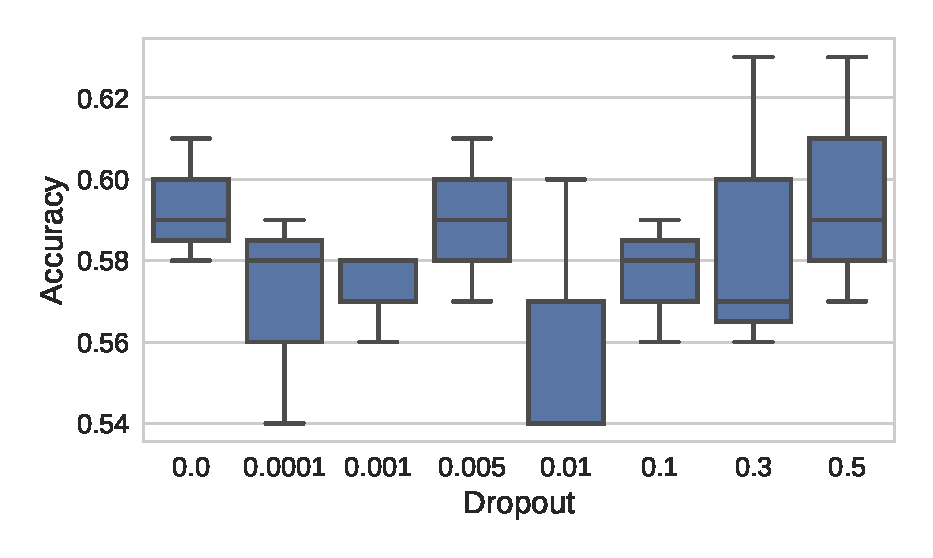
\includegraphics[width=0.9\linewidth]{figures/lstm_dropout.eps}
    \caption{Validation accuracy with different dropout values using 3-fold cross validation for the LSTM model.}
    \label{fig:dropout_LSTM}
\end{figure}


Recurrent Neural Networks (RNN) are neural networks with feedback loops within layers that are able to model and predict long-term patterns in an input signal \cite{Elman90findingstructure}. However, they suffer from the vanishing gradient problem, which limits the information learn in each timestep from its context. As a consequence, LSTM networks were introduced with gated units that control how information from the previous timesteps and how much information from the new sample should be combined \cite{Jozefowicz:2015:EER:3045118.3045367}. The use of a RNN in this work, and concretely a LSTM, is motivated by the fact that EEG signals are highly-dynamic signals that change over time  \cite{LSTM}. Thus, it is expected that a LSTM can capture and model such variations over time.

The architecture used for this model is based on the one presented in \cite{LSTM}, evaluating the performance of models with up to three hidden layers and with 32 to 256 hidden units using 3-fold cross validation. This cross-validation was performed on the raw input data downsampled and without preprocessing. The best-performing architecture was found to be using only 1 layer with 128 hidden units. A higher number of layers or units tended to result in overfitting, while a smaller number underfitted. This is consistent to what could be expected due to the small number of samples. The prediction of the LSTM is produced after processing the whole signal. In addition, to reduce overfitting this layer is followed by a dropout layer. Finally, the output layer uses a softmax activation function with two output units. The final architecture can be found in Figure \ref{fig:archi_LSTM}.

The value for the dropout probability between the LSTM and the fully connected is tuned using 3-fold cross-validation on the downsampled input data without any preprocessing. Figure \ref{fig:dropout_LSTM} shows the results obtained. It can be observed that there is a great variability within the same dropout value. The dropout value is fixed to 0.5, that is one out of two hidden units is dropped. 

\begin{figure}[t]
    \centering
    \includegraphics[width=\linewidth]{figures/CNN_archi.pdf}
    \caption{Our architecture for the CNN model. The kernel size for both convolution layers is 10. The final layer has two output units and uses Sigmoid.}
    \label{fig:archi_CNN}
\end{figure}

\subsection{Convolutional Neural Networks (CNN)}
\label{ssec:methods_CNN}
    The main component of CNNs is the convolutional layer, where the learning of features is attained by convolving a set of filters over the input. Architectures are typically composed of convolutional layers, ReLU or ELU activations, batch normalization, pooling, dropout and fully-connected layers \cite{LSTM}.
    
    CNNs use a variation of multilayer perceptrons designed to require minimal preprocessing \cite{LeNet5}. However, in this work we compare the performance achieved with and without filtering. The architecture used is based on the deep CNN presented in \cite{SchirrmeisterSF17}, reducing the number of hidden layers to prevent overfitting and using ReLU activation layers instead of ELU as shown in Figure \ref{fig:archi_CNN}. After evaluating the performance using a 1D and a 2D convolutional layer for the first layer -- in the first case convoluting only over time, in the second case over time and channels -- we decided to use only 1D convolution over time \cite{BashivanRYC15}. The number of channels produced by the convolution was adjusted using random search and cross-validation.
    
    \begin{figure}[t]
        \centering
        \includegraphics[width=\linewidth]{figures/cnntraintestmatrix.pdf}
        \caption{Validation accuracy for CNN with different dropout probabilities and L2 regularization, considering in each experiment the epoch where the highest average accuracy is obtained.}
        \label{fig:cnntraintestmatrix}
    \end{figure}
    
    After choosing the number of channels we reduced overfitting by adding dropout layers and L2 penalty in the Adam optimizer. The values for both parameters were adjusted as shown in Figure \ref{fig:cnntraintestmatrix}, which presents the results obtained after running 3-fold cross-validation for experiments each with a different value of regularization and dropout probability. The numerical values in the figure have been computed by averaging the learning curves over the three folds, and choosing the epoch with the highest mean in each experiment. From these results we decided to use $0.0316$ for both regularization and dropout probability, since it is the set of parameters for which we have a lowest train accuracy among the ones with highest validation accuracy -- and is therefore less likely to overfit.
% section methods (end)


\section{Results and discussion} % (fold)
\label{sec:results}
	%Intro (mention minibatch size = 100, all with Adam and Cross-Entropy loss), CNN, LSTM, CNN+LSTM
	In this Section we present the results obtained for each of the chosen architectures. All neural network models have been trained using Adam with Cross-Entropy as loss function. The minibatch size used is 25 samples. The trained models are:
	\begin{enumerate}
	    \item Support Vector Machine (SVM).
	    \item Long Short-Term Memory Units (LSTM).
	    \item Convolutional Neural Network (CNN).
	    \item LSTM and CNN combined model.
	\end{enumerate}
	
    \subsection{Baseline - Support Vector Machines (SVM)} % (fold)
    \label{ssec:SVMs}
    We first obtain a baseline for our problem using Support Vector Machines. We evaluate the performance of a system using both a linear and a RBF kernel.  As explained in Section \ref{ssec:methods_SVMs}, both of them have a regularization parameter $C$, while the RBF has in addition $\gamma$. We tune both parameters using 3-fold cross validation on the downsampled training set, both for the linear and the RBF kernel with and without the preprocessing described in Section \ref{ssec:preprocessing}. 
    
    The results from this classifier, as well as the values for $\gamma$ and $C$ obtained can be found in Table \ref{tab:svm}. It can be observed that the best result is obtained with a linear kernel with 73\% accuracy. The performance degrades if the input is preprocessed for both types of kernel. In addition, we show the results using the input samples without downsampling. The accuracy doesn't improve significantly and moreover, it decays in most cases, specially with the RBF kernel. In addition, it should be mentioned that the best results are obtained with the downsampled version of the dataset.
    
    \begin{table}[t]
        \centering
        \caption{Parameters and accuracy using SVM. 100 Hz refers to the downsampled version of the dataset and 1 kHz to version without downsampling.}
        \label{tab:svm}
        \begin{tabular}{ccccc}
        \hline
         &  & \multirow{2}{*}{\textbf{Parameters}} & \multicolumn{2}{c}{\textbf{Accuracy (\%)}} \\
         &  &  & \textbf{100 Hz} & \textbf{1 kHz} \\ \hline
        \multirow{2}{*}{\textbf{Linear}} & \textbf{Without preprocessing} & $C = 0.0001$ & 73 & 74 \\ \cline{2-5} 
         & \textbf{With preprocessing} & $C = 1$ & 66 & 60 \\ \hline
        \multirow{2}{*}{\textbf{RBF}} & \textbf{Without preprocessing} & \begin{tabular}[c]{@{}c@{}}$C =10000$\\ $\gamma = 1e-05$\end{tabular} & 63 & 49 \\ \cline{2-5} 
         & \textbf{With preprocessing} & \begin{tabular}[c]{@{}l@{}}$C =10000$\\ $\gamma = 1e-04$\end{tabular} & 65 & 57 \\ \hline
        \end{tabular}
    \end{table}
    
    \subsection{Long Short-Term Memory Units (LSTM)} % (fold)
    \label{ssec:LSTM}
    The LSTM is trained with Adam as optimizer. The learning rate is set to 0.001 and the decay rates of the first and second moments are 0.9 and 0.999 respectively, as recommended in \cite{adam}. Different values for these parameters as well as for the L2 penalty were evaluated with no improvement in the performance. 
    
    We study the performance of this model with the architecture presented in Section \ref{ssec:methods_LSTM} using both the data downsampled to 100 Hz and with 1 kHz sampling rate and with and without filtering, so we can compare the effect these parameters have. Figure \ref{fig:lstm_50} shows the results with 100 Hz while Figure \ref{fig:lstm_500} shows the results with 1 kHz after training for 60 epochs. In both cases, the models are trained five times and the mean result per epoch and 95\% confidence interval presented. With 100 Hz the best accuracy, around 60\% accuracy, is obtained with the filtered data. On the other hand, the performance decreases with 1 kHz as sampling rate, reaching only 55\% accuracy with both filtered and non-filtered data. This is consistent with what one could expect from LSTMs, since they usually benefit from shorter time sequences \cite{LSTM}. Hence, with the higher sampling rate the model tends to learn less, especially with filtering, where the model performance decreases as the number of epochs grow. A possible cause is that filtering removes information from the data, making it easier to overfit. 
    
    In comparison to our baseline, this model achieves worse accuracies and it's clearly outperformed.
    
    
    \begin{figure}[t]
        \begin{subfigure}{0.5\textwidth}
            \centering
            \includegraphics[width=\textwidth]{figures/lstm_50.pdf}
            \caption{Accuracy with 100 Hz data.}
            \label{fig:lstm_50}
        \end{subfigure}
        \begin{subfigure}{0.5\textwidth}
            \centering
            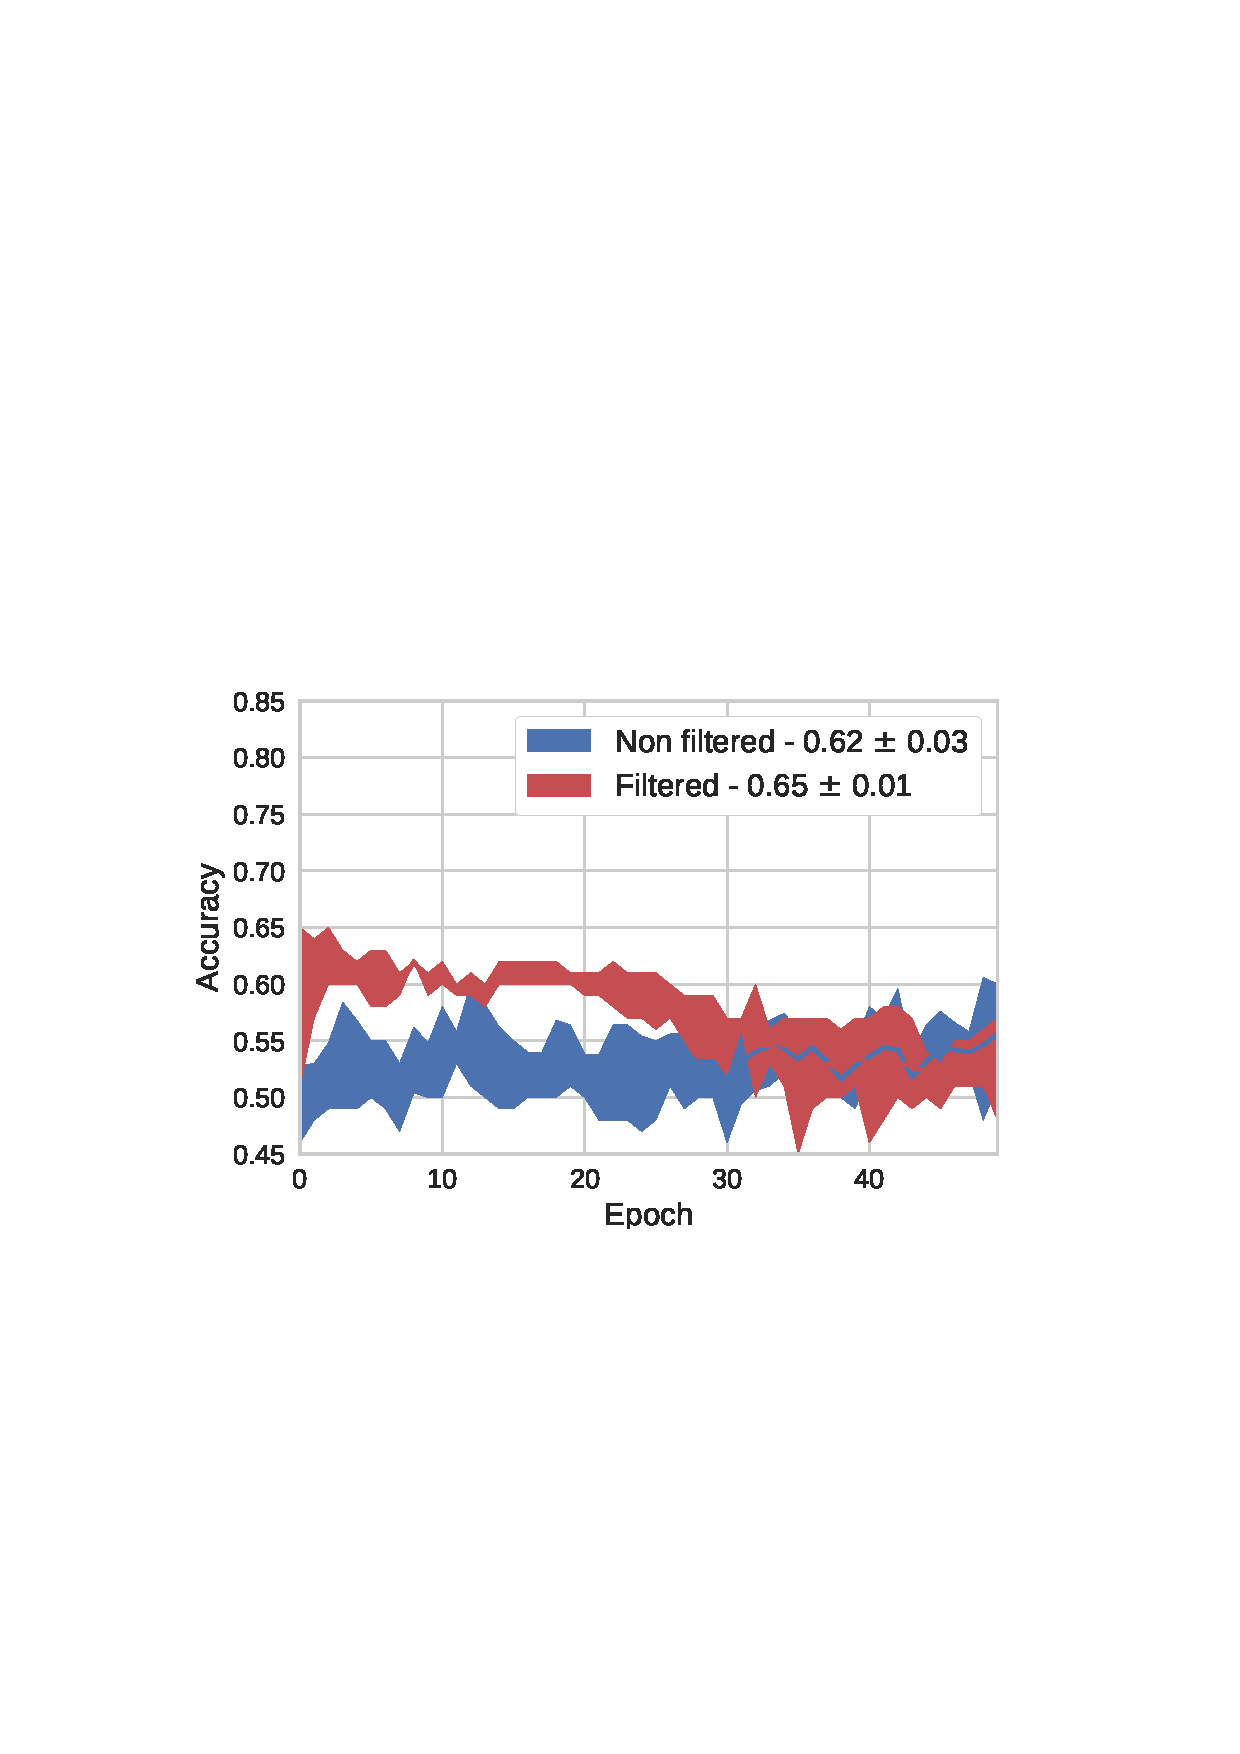
\includegraphics[width=\textwidth]{figures/lstm_500.pdf}
            \caption{Accuracy with 1 kHz data.}
            \label{fig:lstm_500}
        \end{subfigure}
        \caption{Accuracy of the LSTM model for the downsampled and full versions of the dataset training the model five times. In deeper blue and red are the mean values, while in lighter colors are the 95\% confidence intervals.}
        \label{fig:perf_optim}
    \end{figure}
  

    \subsection{Convolutional Neural Network (CNN)} % (fold)
    \label{ssec:CNN}
    We study the performance of the CNN model with the architecture presented in Section \ref{ssec:methods_CNN}. Similarly to the analysis carried out in Section \ref{ssec:LSTM}, we train with Adam using the same parameters as before for the data with 100 Hz and 1 kHz sampling rates and with and without filtering. Figure \ref{fig:cnn_50} shows the results with 100 Hz while Figure \ref{fig:cnn_500} shows the results with 1 kHz after training for 200 epochs.

    \begin{figure}[t]
        \begin{subfigure}{0.5\textwidth}
            \centering
            \includegraphics[width=\textwidth]{figures/cnn_50.pdf}
            \caption{Accuracy with 100 Hz data.}
            \label{fig:cnn_50}
        \end{subfigure}
        \begin{subfigure}{0.5\textwidth}
            \centering
            \includegraphics[width=\textwidth]{figures/cnn_500.pdf}
            \caption{Accuracy with 1 kHz data.}
            \label{fig:cnn_500}
        \end{subfigure}
        \caption{Accuracy of the CNN model for the downsampled and full versions of the dataset training the model five times. In deeper blue and red are the mean values, while in lighter colors are the 95\% confidence intervals.}
        \label{fig:cnn_perf_optim}
    \end{figure}
    

    In all cases the accuracy is between 70\% and 80\% for the non-filtered data, and around 60\% for the filtered one. The reason for this is that the CNN is able to learn the features from the training data better than the LSTM. By filtering the input signals we are removing information, resulting in a worse performance of the CNN. We can also note that for 1 kHz data, filtering causes the model to overfit -- as seen from the accuracy decrease around epoch 100 for the filtered curve in Figure \ref{fig:cnn_500}.
    
    When comparing the accuracies obtained for the non filtered, downsampled and non-downsampled data, we can observe that it is considerably similar for both. It is worth noting that the parameters chosen for the model had been optimized for the downsampled training dataset, so the fact that the accuracy is similar shows the robustness of the CNN model.
    
    This model achieves better accuracies than both the LSTM model and the baseline.
    
    

    \subsection{LSTM and CNN combined model} % (fold)
    \label{ssec:CNN+LSTM}
    
        \begin{figure}[t]
            \centering
            \includegraphics[width=0.5\textwidth]{figures/lstm_cnn_50.pdf}
            \caption{Accuracy of the LSTM and CNN combined model for the downsampled and full versions of the dataset training the model five times. In deeper blue and red are the mean values, while in lighter colors are the 95\% confidence intervals.}
            \label{fig:cnn_lstm_50}
        \end{figure}
    In addition to the previous experiments, we combine the CNN and LSTM models. Both models are trained on parallel with the architecture described on Sections \ref{ssec:methods_LSTM} and \ref{ssec:methods_CNN}, removing the final fully connected of each model. Instead, the results from both models are concatenated and a final fully connected layer with Sigmoid as activation function is added to obtain the output. 
    
    The resulting model is trained with 0.032 L2-regularization using non-filtered data with 100 Hz and 1 Khz sampling rate. Since it has been found that the filtering is, in general, detrimental to the performance, we do not report the accuracies with this preprocessing.
    
    The accuracy obtained can be found in Figure \ref{fig:cnn_lstm_50}. It can be observed that the result is almost the same with the downsampled and full versions of the dataset. Both obtain accuracies close to 80\%, with the downsampled version performing slightly better. These values are similar to the ones reached using only CNN and no clear improvements can be observed.
    
    For completeness, Figure \ref{fig:traintestcomb} shows the training and test accuracy curves for the signal downsampled to 100 Hz. We can see that the model does not seem to learn much after 125 epochs, which prevents it from overfitting but may indicate that the learning capacity of the model could be improved.
    
        \begin{figure}[t]
            \centering
            \includegraphics[width=0.5\textwidth]{figures/traintestcomb.pdf}
            \caption{Train and test accuracy of the LSTM and CNN combined model for the downsampled input signals after training the model five times. In deeper black and blue are the mean values for train and test respectively, while in lighter colors are the 95\% confidence intervals.}
            \label{fig:traintestcomb}
        \end{figure}

% section results (end)

\section{Conclusions} % (fold)
\label{sec:conclusions}
    % Filtering no mejora
    % LSTM se va a la mierda
    In this project we proposed different solutions for predicting the laterality of finger movements. Our final model was a combination of CNN and LSTM predictors, which results in a model that achieves between 70\% and 80\% accuracy. These values are similar to what we achieved using the model based on CNN, with the advantage that the combined model was more robust and performed similarly for signals both with 100 Hz and 1 kHz sampling frequencies. We could also verify that there was not a clear advantage of using a higher sampling frequency, which increments the complexity. Nevertheless, the proposed models generally perform better when using input signals downsampled to 100 Hz.
    
    Regarding preprocessing, we initially considered filtering and normalizing the input signals as well as reducing the initial number of electrodes. Neither of these techniques resulted in better results, since reducing the amount of information in the signals reduced the accuracy of the models.
    
    	
	Future work could include using the CNN to obtain a series of features that could be used as inputs to a LSTM. In addition, the parameters of our models should be tuned trying more combinations, which would probably increase the accuracy -- particularly for the combined model.
        
% section summary (end)

\bibliographystyle{IEEEtran}
\bibliography{literature}

\end{document}
